\documentclass[11pt,a4paper]{article}
\usepackage[margin=24mm]{geometry}
\usepackage[T1]{fontenc}
\usepackage{lmodern}
\usepackage{amsmath,amssymb,booktabs,graphicx}
\usepackage[colorlinks=true,linkcolor=blue,urlcolor=blue]{hyperref}
\title{Daniel versus Marcolino\\threefold initial-error simulation}
\author{Numerical study note}
\date{}

\begin{document}
\maketitle

\begin{abstract}
This note compares two ways to condition the same LQR switching-time command on the article's three-cell converter. It uses an initial displacement from the nominal orbit three times as large as the article's initial displacement. Daniel keeps the final boundary fixed and scales all interior offsets; Marcolino delays switches sequentially and can extend a cycle. Its moving-anchor and fixed-clock errors must be read separately.
\end{abstract}

\section{Question and experimental setup}

The two trial runs hold the plant, gain, initial condition, reference orbit, mode sequence, and dwell limit fixed. Only the actuator-side conditioner changes. The article's benchmark has nine mode intervals per cycle, nominal period $T=286\,\mu\mathrm{s}$, and minimum applied dwell $d_{\min}=3\,\mu\mathrm{s}$. For this study we triple the displacement of the article's original initial state from the nominal orbit anchor:
\[
 x_0^{(3)}=\bar x_0+3\bigl(x_0^{\rm article}-\bar x_0\bigr)
 =\begin{bmatrix}2.6935&23.8777&-1.8704\end{bmatrix}^{\!\top}.
\]
The normalized initial error is $2.951839$, three times its article value. The same aggressive LQR gain uses normalized input weight $0.001I$. This starting current is negative; the ideal switched-affine model propagates it, but the trial does not establish physical validity for hardware that forbids reverse current. At each \emph{actual} cycle start the controller requests an eight-component switching-time offset vector $\delta^{\rm raw}_k=-K(x_k-\bar x_0)$, where $\bar x_0$ is the nominal orbit anchor. Both runs propagate the same exact switched-affine converter dynamics for 100 cycles. The gain is not redesigned when a cycle is prolonged.

Daniel's rule, the article's method, multiplies every component of $\delta^{\rm raw}_k$ by a single maximal feasible factor $\beta_k\in[0,1]$. The first and final cycle boundaries stay fixed, so every realized cycle lasts $T$. In the Marcolino comparison, a sequential-delay adaptation of their Algorithm~1, the realized interior switching times relative to the current cycle start obey
\begin{align}
 t_0&=\bar t_0,\\
 t_i&=\max\{\bar t_i+\delta^{\rm raw}_{k,i},\ t_{i-1}+d_{\min}\},
       &&i=1,\ldots,8,\\
 t_9&=\max\{\bar t_9,\ t_8+d_{\min}\}.
\end{align}
The next cycle starts at $t_9$, which can be later than the nominal boundary. This is an \emph{adaptation} of their actuator rule to our converter: Marcolino et al. study switched actuators of an LTI plant, whereas this benchmark has mode-dependent state dynamics. It is not a numerical reproduction of their paper.\footnote{M.~H.~Marcolino, R.~K.~H.~Galv\~ao, and K.~H.~Kienitz, ``Predictive Control of Linear Systems with Switched Actuators Subject to Dwell-Time Constraints,'' \emph{Journal of Control, Automation and Electrical Systems} 32, 2021, Algorithm~1. \url{https://doi.org/10.1007/s40313-020-00667-9}.}

\section{Two clocks, two error measures}

Let $s_k$ be the elapsed physical time at the start of cycle $k$. The study reports the normalized error against the orbit anchor at that actual cycle start,
\begin{equation}
 E_{\rm reset}(k)=\bigl\|S_x^{-1}\bigl(x(s_k)-\bar x_0\bigr)\bigr\|_2,
\end{equation}
and the normalized error against the originally clocked periodic reference at the same physical time,
\begin{equation}
 E_{\rm global}(k)=\bigl\|S_x^{-1}\bigl(x(s_k)-\bar x(s_k\bmod T)\bigr)\bigr\|_2.
\end{equation}
Here $S_x$ is the state-normalization matrix used in the article. The original nominal within-cycle dynamics generate $\bar x(\cdot)$. The first measure tests proximity to a fixed \emph{point in state space} at each method's own cycle start. It treats Marcolino's delayed start as a new reference anchor. The second tests the original \emph{clocked trajectory} at the actual sample time. They agree for Daniel's fixed-period schedule but need not agree for Marcolino. Both errors are sampled at actual cycle starts, not at a common grid of physical times. Thus a smaller $E_{\rm reset}$ does not, by itself, establish faster tracking of the original reference.

The middle panel of Figure~\ref{fig:comparison} reports each realized cycle duration,
\begin{equation}
 D_k=s_k-s_{k-1}.
\end{equation}
If Marcolino delays a final switch, $D_k$ exceeds the nominal $T=286\,\mu\mathrm{s}$. As conditioning becomes unnecessary, later durations return to $T$. This is \emph{not} a recovery of the original clock: the boundary offset $s_k-kT=\sum_{j=1}^k(D_j-T)$ remains after any earlier excess duration. Its effect on the periodic fixed-clock error depends on the remaining offset modulo $T$; even an offset near one whole period can produce a small fixed-clock error without recovering the original schedule.

\section{Numerical result}

\begin{table}[ht]
\centering
\caption{Threefold initial-error trial with the same gain and initial state for both policies. Threshold crossings use normalized error $0.01$ at each method's own cycle starts, not a shared physical-time grid.}
\label{tab:comparison}
\small
\setlength{\tabcolsep}{3pt}
\begin{tabular}{@{}p{.63\linewidth}p{.14\linewidth}p{.18\linewidth}@{}}
\toprule
Measure & Daniel & Marcolino\\
\midrule
Minimum realized dwell, $\mu\mathrm{s}$ & 3 & 3\\
Cycles with conditioning active & 10 & 5\\
Cycles extending beyond $T$ & 0 & 4\\
First-cycle duration, $\mu\mathrm{s}$ & 286 & 462.479\\
Cycle duration from cycle 5, $\mu\mathrm{s}$ & 286 & 286\\
First sustained $E_{\rm reset}<0.01$ & cycle 12 & cycle 7\\
Elapsed time at own crossing, ms & 3.432 & 2.293\\
$E_{\rm reset}$ at cycle 100 & $2.07\cdot10^{-15}$ & $1.71\cdot10^{-15}$\\
$E_{\rm global}$ at cycle 100 & $2.07\cdot10^{-15}$ & $0.004936$\\
First sustained $E_{\rm global}<0.01$ & cycle 12 & cycle 8\\
\bottomrule
\end{tabular}
\end{table}

Tripling the article's initial error triples the first raw LQR action. Daniel's first-cycle factor falls from $0.293978$ to $\beta_0=0.097993$, so its first \emph{applied} schedule is unchanged. Daniel has $\beta_k<1$ during ten cycles here, versus three in the original-state run. Its final boundary remains fixed at $286\,\mu\mathrm{s}$ in every cycle. Marcolino's first cycle lasts $462.479\,\mu\mathrm{s}$ and its next three also exceed $286\,\mu\mathrm{s}$.

At Marcolino's seventh boundary, $s_7=2.2930\,\mathrm{ms}$, $E_{\rm reset}(7)=0.00648$ is below $0.01$, while $E_{\rm global}(7)=0.01067$ is above it; the fixed-clock error first stays below $0.01$ at its eighth boundary. Marcolino's four extended cycles add $291.038\,\mu\mathrm{s}$, one nominal period plus $5.038\,\mu\mathrm{s}$. Its small late fixed-clock error partly reflects this phase wrap, not a return to the original switching schedule. These crossings are measured at each method's own cycle starts.

\begin{figure}[ht]
\centering
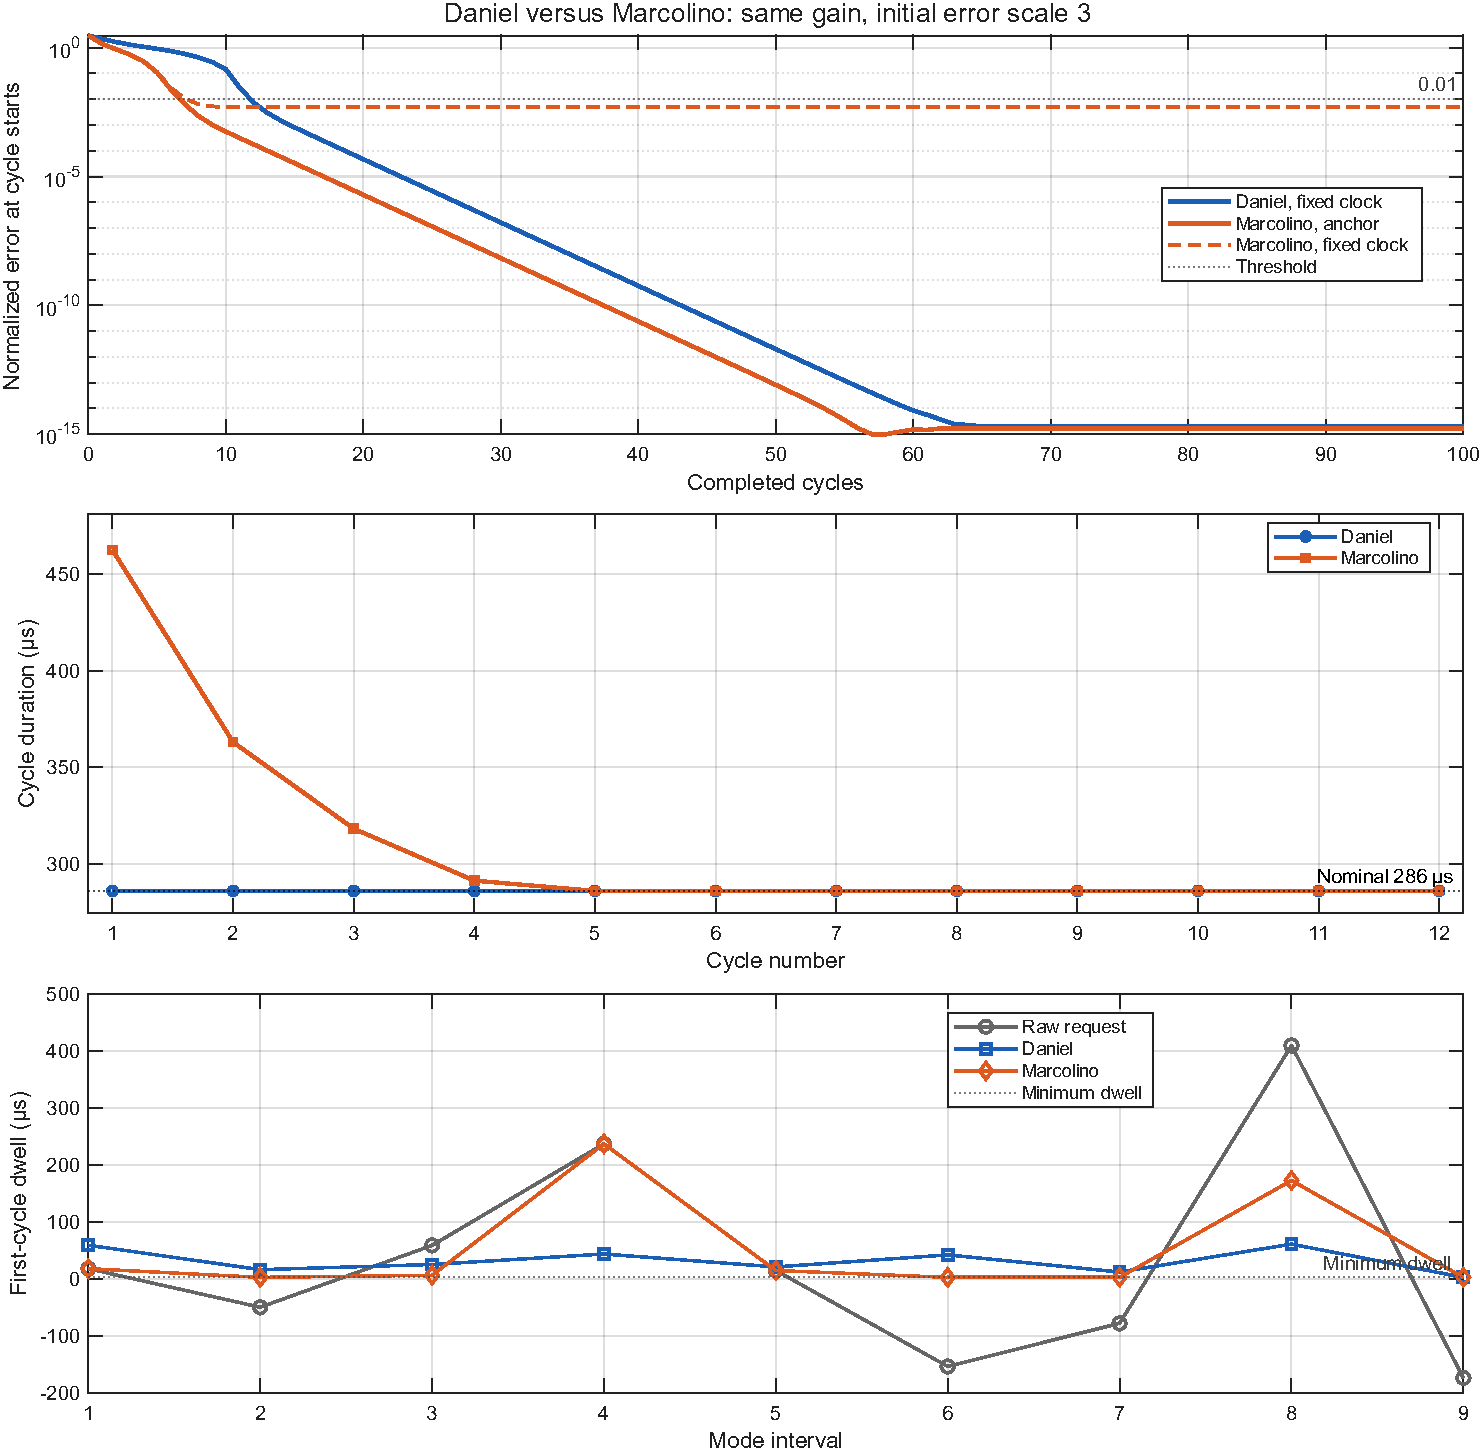
\includegraphics[width=.95\linewidth,height=.69\textheight,keepaspectratio]{../results/error-scale-3x/comparison.pdf}
\caption{Threefold initial-error run. Top: moving-anchor and fixed-clock errors for Daniel and Marcolino. Middle: the first 12 cycle durations. Bottom: requested and realized first-cycle dwells. Daniel keeps the last boundary fixed; both applied schedules satisfy the $3\,\mu\mathrm{s}$ dwell bound.}
\label{fig:comparison}
\end{figure}

\subsection{Extending the article's early-response figure}

The article's Figure~4 originally compares Daniel with open loop over the first 25 cycles. The user-supplied raster of that figure is kept unchanged in the study's \texttt{reference} directory; it contains no Marcolino run. Figure~\ref{fig:article-extended} is a study figure that adds Marcolino to this early-response view. Its error panel distinguishes Marcolino's moving-anchor and original-clock errors. The middle panel shows Daniel's beta. It cannot show a Marcolino beta because sequentially delayed switches do not share a common factor; a separately labeled right axis counts the postponed switches. The lower panel compares both requested and realized minimum dwells. The open-loop trace uses this trial's tripled initial error. It is not the article's original-state trace.

\begin{figure}[p]
\centering
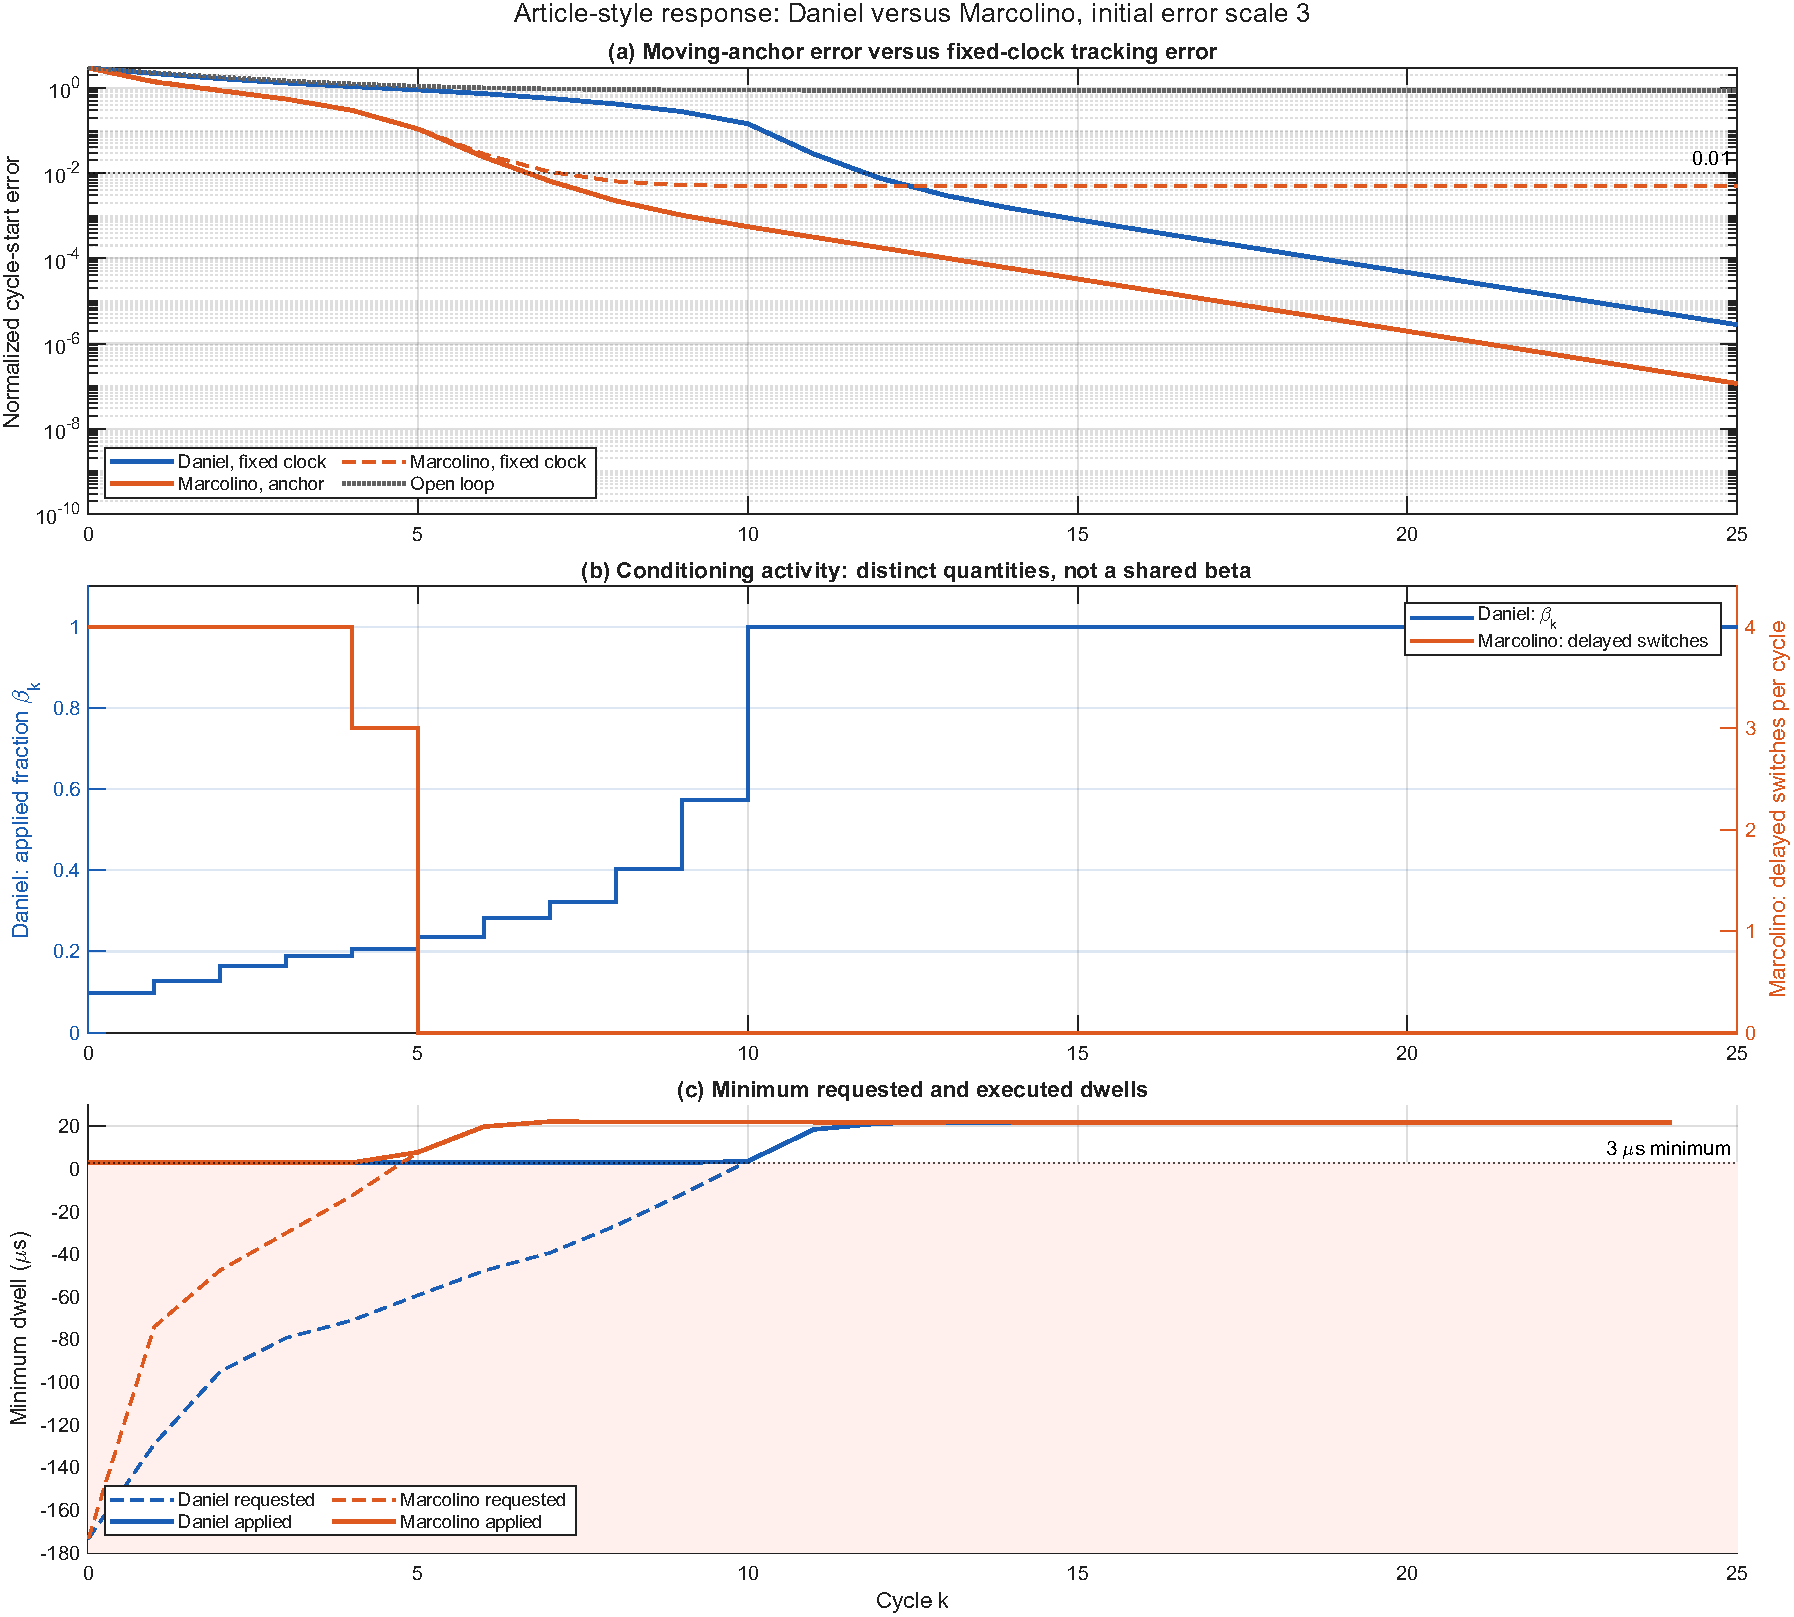
\includegraphics[width=\linewidth,height=.78\textheight,keepaspectratio]{../results/error-scale-3x/article_response_with_marcolino.pdf}
\caption{Threefold initial-error response over 25 cycles. Blue is Daniel and orange Marcolino. Panel (b) shows Daniel's factor below one for the first ten cycles, then at one; Marcolino's right axis counts delayed switches instead. Both applied schedules meet the $3\,\mu\mathrm{s}$ bound in panel (c).}
\label{fig:article-extended}
\end{figure}

\section{Continuous-time trajectories}

Figure~\ref{fig:states} compares both exact state trajectories against the original reference periodic trajectory. It uses the first 12 nominal periods, $0\le t\le 3.432\,\mathrm{ms}$, on a \emph{common physical-time axis}. The state-space panel traces the three converter states, while the other panels plot their waveforms against time. Daniel is blue, Marcolino orange, and the original fixed-clock reference dashed black. Each response uses 30 exact samples per mode interval. The two response grids have different switching instants; the figure neither aligns their samples by cycle index nor interpolates one response onto the other. The accompanying \texttt{trajectory\_samples.csv} retains the sampled values through each method's twelfth complete cycle, including the later end of Marcolino's twelfth cycle.

In three-dimensional state space the methods approach the same periodic orbit. The time plots show different transients against a common physical-time reference. Marcolino's late waveform nearly aligns with that reference because its accumulated extensions approach one complete nominal period. It does not shorten subsequent cycles to regain the original schedule. The trajectory figure is simulation evidence, not a stability proof.

\begin{figure}[p]
\centering
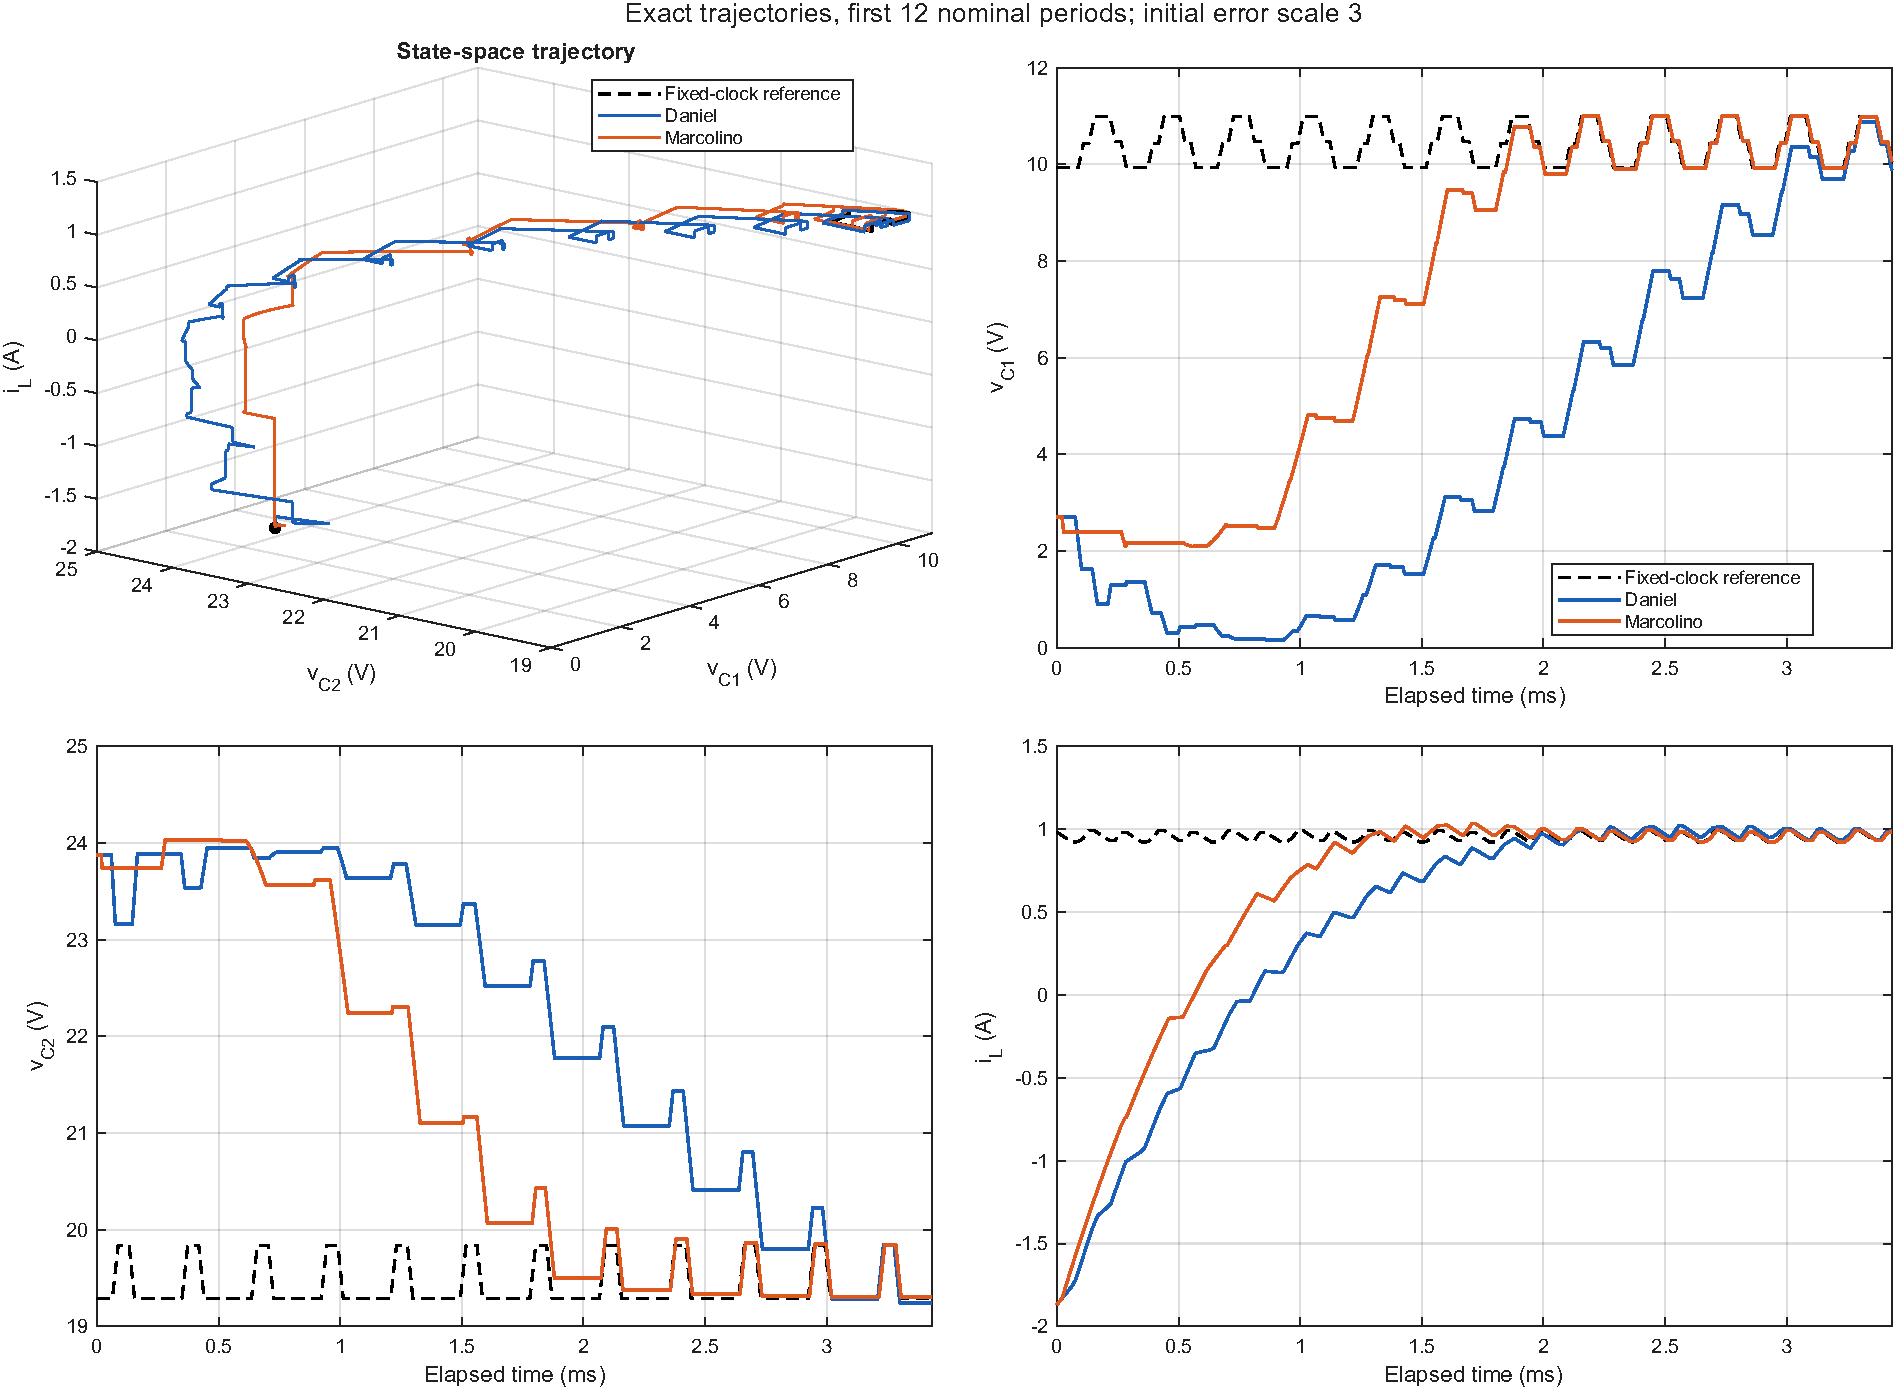
\includegraphics[width=\linewidth,height=.78\textheight,keepaspectratio]{../results/error-scale-3x/state_trajectories.pdf}
\caption{Exact trajectories of the same mode-dependent converter under Daniel and Marcolino. Upper left: state-space paths. Other panels: physical states versus the same elapsed-time clock, with the original fixed-period reference. The plotted window is the first 12 nominal periods; the sampled records are not resampled onto a common grid.}
\label{fig:states}
\end{figure}

\section{What the comparison does and does not establish}

The comparison isolates how two conditioners handle the same raw LQR command. Daniel scales the complete command to keep the final boundary and period fixed. Marcolino delays switches sequentially and may extend the cycle. The difference in clock behavior is material for a fixed-frequency converter and for tracking an externally timed reference. The cycle-sampled squared-error total stored in the study's CSV compares samples taken at different physical times, so it should not be treated as a common-clock performance cost.

This is a deterministic simulation from one initial condition over 100 cycles. The mode-dependent converter is outside the plant class for which Marcolino et al. originally formulated their method. The article's common-quadratic Lyapunov certificate covers Daniel's fixed-period \emph{linearized} family, not Marcolino's extended-cycle map. The exact switched-affine trajectories shown here are numerical evidence; they do not prove a general nonlinear stability claim or establish that either conditioner is always preferable.

\paragraph{Reproducibility.} Run \texttt{run\_comparison([],3)} as described in the parent study's \texttt{README.md}. This report uses only figures and numbers from \texttt{results/error-scale-3x}. The article's original-state figures remain unchanged elsewhere in the study.

\end{document}
